%%%%%%%%%%%%%%%%%%%%%%%%%%%%%%%%%%%%%%%%%
% University Assignment Title Page 
% LaTeX Template
% Version 2.1 (18/10/18)
% Modified by
% Erdem TUNA &
% Halil TEMURTAŞ &
% Enes TAŞTAN
%%%%%%%%%%%%%%%%%%%%%%%%%%%%%%%%%%%%%%%%%
%
%----------------------------------------------------------------------------------------
%	PACKAGES AND OTHER DOCUMENT CONFIGURATIONS
%----------------------------------------------------------------------------------------
\documentclass[a4paper,12pt]{article}
%-----packages------
\usepackage[a4paper, total={6.2in, 8.4in}]{geometry}
\usepackage[english]{babel}
\usepackage[utf8x]{inputenc}
\usepackage{amsmath}
\usepackage{graphicx}
\usepackage[colorinlistoftodos]{todonotes}
\usepackage{gensymb} % this could be problem
\usepackage{float}
\usepackage{fancyref}
\usepackage{subcaption}
\usepackage[toc,page]{appendix} %appendix package
\usepackage{xcolor}
\usepackage{listings}
\usepackage{xspace}
\usepackage{amssymb}
\usepackage{nicefrac}
\usepackage{gensymb}
\usepackage{fancyhdr}
\usepackage{blindtext}  % for dummy text, use \blindtext or \BlindText
\usepackage[final]{pdfpages}  % pdf include
\usepackage{array} %allows more options in tables
\usepackage{pgfplots,pgf,tikz} %coding plots in latex
\usepackage{capt-of} % allows caption outside the figure environment
\usepackage[export]{adjustbox} %more options for adjusting the images
\usepackage{multicol,multirow,slashbox} % allows tables like table1
%\usepackage[hyperfootnotes=false]{hyperref} % clickable references
\usepackage{epstopdf} % useful when matlab is involved
%\usepackage{placeins} % prevents the text after figure to go above figure with \FloatBarrier 
%\usepackage{listingsutf8,mcode} %import .m or any other code file mcode is for matlab highlighting

%-----end of packages

%-----specifications-----
\definecolor{mGreen}{rgb}{0,0.6,0} % for python
\definecolor{mGray}{rgb}{0.5,0.5,0.5}
\definecolor{mPurple}{rgb}{0.58,0,0.82}
\definecolor{mygreen}{RGB}{28,172,0} % color values Red, Green, Blue for matlab
\definecolor{mylilas}{RGB}{170,55,241}

\setcounter{secnumdepth}{5} % how many sectioning levels to assign numbers to
\setcounter{tocdepth}{5}    % how many sectioning levels to show in ToC

\lstdefinestyle{CStyle}{
	commentstyle=\color{mGreen},
	keywordstyle=\color{magenta},
	numberstyle=\tiny\color{mGray},
	stringstyle=\color{mPurple},
	basicstyle=\footnotesize,
	breakatwhitespace=false,         
	breaklines=true,
	frame=single,
	rulecolor=\color{black!40},                 
	captionpos=b,                    
	keepspaces=true,                 
	numbers=left,                    
	numbersep=5pt,                  
	showspaces=false,                
	showstringspaces=false,
	showtabs=false,                  
	tabsize=2,
	language=C
}

\lstset{language=Matlab,%
	%basicstyle=\color{red},
	breaklines=true,%
	frame=single,
	rulecolor=\color{black!40},
	morekeywords={matlab2tikz},
	keywordstyle=\color{blue},%
	morekeywords=[2]{1}, keywordstyle=[2]{\color{black}},
	identifierstyle=\color{black},%
	stringstyle=\color{mylilas},
	commentstyle=\color{mygreen},%
	showstringspaces=false,%without this there will be a symbol in the places where there is a space
	numbers=left,%
	numberstyle={\tiny \color{black}},% size of the numbers
	numbersep=9pt, % this defines how far the numbers are from the text
	emph=[1]{for,end,break},emphstyle=[1]\color{red}, %some words to emphasise
	%emph=[2]{word1,word2}, emphstyle=[2]{style},    
}


\tikzset{
	desicion/.style={
		diamond,
		draw,
		text width=4em,
		text badly centered,
		inner sep=0pt
	},
	block/.style={
		rectangle,
		draw,
		text width=10em,
		text centered,
		rounded corners
	},
	cloud/.style={
		draw,
		ellipse,
		minimum height=2em
	},
	descr/.style={
		fill=white,
		inner sep=2.5pt
	},
	connector/.style={
		-latex,
		font=\scriptsize
	},
	rectangle connector/.style={
		connector,
		to path={(\tikztostart) -- ++(#1,0pt) \tikztonodes |- (\tikztotarget) },
		pos=0.5
	},
	rectangle connector/.default=-2cm,
	straight connector/.style={
		connector,
		to path=--(\tikztotarget) \tikztonodes
	}
}

\tikzset{
	desicion/.style={
		diamond,
		draw,
		text width=4em,
		text badly centered,
		inner sep=0pt
	},
	block/.style={
		rectangle,
		draw,
		text width=10em,
		text centered,
		rounded corners
	},
	cloud/.style={
		draw,
		ellipse,
		minimum height=2em
	},
	descr/.style={
		fill=white,
		inner sep=2.5pt
	},
	connector/.style={
		-latex,
		font=\scriptsize
	},
	rectangle connector/.style={
		connector,
		to path={(\tikztostart) -- ++(#1,0pt) \tikztonodes |- (\tikztotarget) },
		pos=0.5
	},
	rectangle connector/.default=-2cm,
	straight connector/.style={
		connector,
		to path=--(\tikztotarget) \tikztonodes
	}
}
%-----end of specifications-----


%----commands----
\newcommand\nd{\textsuperscript{nd}\xspace}
\newcommand\rd{\textsuperscript{rd}\xspace}
\newcommand\nth{\textsuperscript{th}\xspace} %\th is taken already
\newcommand{\specialcell}[2][c]{ \begin{tabular}[#1]{@{}c@{}}#2\end{tabular}} % for too long table lines

\newcommand{\blankpage}{
	\- \\[9cm]	
	{ \centering \textit{This page intentionally left blank.} \par }
	\- \\[9cm]
}% For Blank Page

\makeatletter
\renewcommand\paragraph{\@startsection{paragraph}{4}{\z@}%
	{-2.5ex\@plus -1ex \@minus -.25ex}%
	{1.25ex \@plus .25ex}%
	{\normalfont\normalsize\bfseries}}
\makeatother
%-----end of commands-----

\begin{document}

\begin{titlepage}

\newcommand{\HRule}{\rule{\linewidth}{0.5mm}} % Defines a new command for the horizontal lines, change thickness here
\centering 


\includegraphics[width=\textwidth,height=\textheight,keepaspectratio]{images/logo3-with-stroke}\\[1cm]

\textsc{\LARGE Middle East Technical University}\\[1.5cm] % Name of your university/college
\textsc{\Large Department of \\Electrical and Electronics Engineering }\\[0.5cm] % Major heading such as course name
\textsc{\large EE493 ENGINEERING DESIGN I}\\[0.5cm] % Minor heading such as course title


\HRule \\[0.4cm]
{ \huge \bfseries  Business Statement Report}\\[0cm] % Title of your document
\HRule \\[1cm]

\begin{minipage}{\textwidth}
\begin{flushleft}
	\large{\textbf{Supervisor\hspace{1.55cm}:}}	Assoc. Prof. Emre Özkan (Section 6)\\
	\large{\textbf{Company Name :}}	Duayenler Ltd. Şti.\\
	\large{\textbf{Members\hspace{1.89cm}:}}
	Sarper Sertel, 2094449 (Contact Person) \\\hspace{4.39cm} 
	Enes Taştan, 2068989 \\\hspace{4.39cm} 
	Erdem Tuna, 2617419 \\\hspace{4.39cm} 
	Halil Temurtaş, 2094522 \\\hspace{4.39cm} 
	İlker Sağlık, 2094423   \\
\end{flushleft}
\end{minipage}\\[1cm]

\begin{flushbottom}
{\large October 19, 2018}\\[1cm] % Date, change the \today to a set date if you want to be precise
\end{flushbottom}

\end{titlepage}

%\blankpage
\tableofcontents
\newpage

%Enes uses \qquad instead of \-\indent he thinks that it is simpler. Just a thought though

\section{Introduction}
	In this report, we will give the general information about our company, DUAYENLER Ltd. Şti., and us as co-founders of the company. This report, also contains our basic understandings of the four possible Capstone projects in brief details.
	
\section{About the Company}
	Founded in September 2018 by five electrical engineering students from Middle East Technical University, DUAYENLER Ltd. Şti. is a promising new robotics start-up company.

\subsection{Our Mission}
Our mission is to design products for real life problems by creating innovative solutions.
	
\subsection{Our Mission}
Our vision is to be frontier in robotics by intelligently automating the future world.

\section{About Us}
	\textbf{DUAYENLER Ltd. Şti.} was founded in September 2018 by 5 Co-founders ,namely, Sarper Sertel, Enes Taştan, Erdem Tuna, Halil Temurtaş \& İlker Sağlık.   Although all of the co-founders are from similar backgrounds and some of them even have long-lasting pair-relationships, the efforts of the Sarper Sertel brought  the group together to establish the company.  In this section, we will introduce ourselves as the co-founders of DUAYENLER. \\%[0.2cm]

%The co-founders can be seen from \textit{Figure~\ref{fig:meeting_foto}}.

%\begin{figure}[H]
%	\center
%	\setlength{\unitlength}{\textwidth} 
%	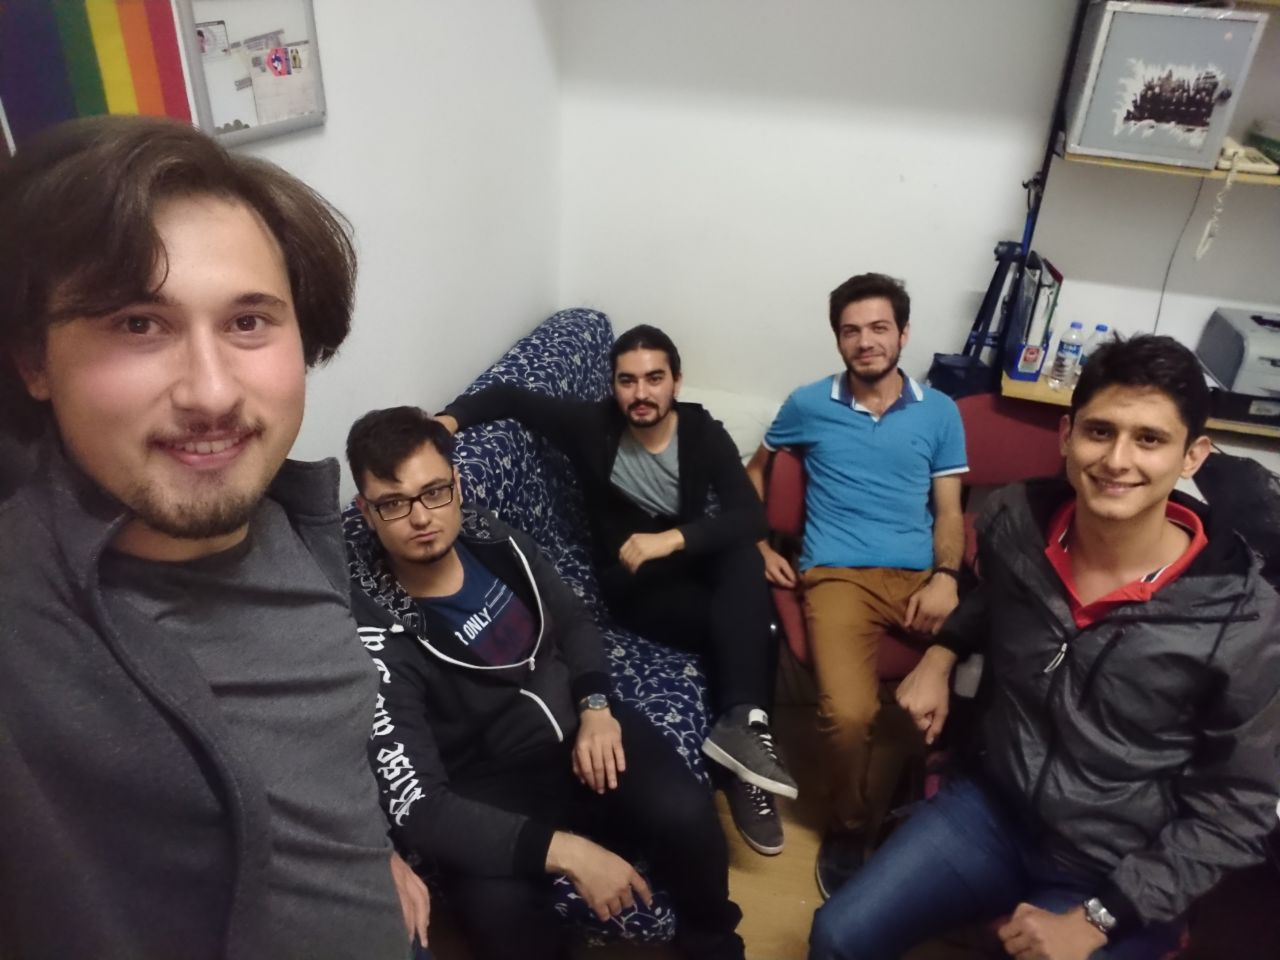
\includegraphics[width=0.7\unitlength]{images/meeting2}
%	\caption{\label{fig:meeting_foto} \small The Co-Founders of DUAYENLER Ltd. Şti. }
%\end{figure}


%------Sarper-----------

\begin{minipage}{0.33\textwidth}
\begin{flushleft} \large

\begin{figure}[H]
	\center
	\setlength{\unitlength}{\textwidth} 
	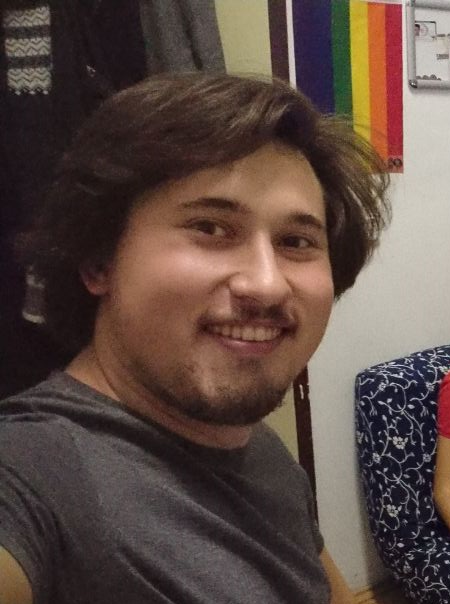
\includegraphics[width=0.8\unitlength]{images/sarper_foto}
	\caption{\label{fig:sarper_foto} \small Sarper SERTEL }
\end{figure}


\end{flushleft}
\end{minipage}
\begin{minipage}{0.66\textwidth}
\begin{flushleft} 

	As a person bringing group together, Sarper Sertel was laboratory pair with Enes for EE214 \& EE313 and was pair with İlker for EE314 laboratory course. He was also project partner with Erdem \& Halil for EE302 Project im which they called themselves Group Duayenler. As a graduation student, he chose the \textbf{Electronics} option. And as an engineering student, he has specialized in number of topics such as:
	
\begin{itemize}
	\item Analog Circuit Design
	\item Digital Circuit Design
	\item Expert LtSpice User
	\item Advance Matlab User
\end{itemize}


\end{flushleft}
\end{minipage}\\[0.4cm]

	More information about Sarper SERTEL can be accessed from his curriculum vitae at APPENDIX.\\[0.4cm]

%-------Enes----------

\begin{minipage}{0.66\textwidth}
\begin{flushleft} 

	Enes Taştan, an Electronics and Physics double-major students, interested in physical \& theoretical aspects of electronics engineering as well as real-life applications of them thanks to his summer-practice knowledge. Due to his physics courses, he is planning to graduate next year but he is planning to chose \textbf{Electronics} option. As an engineering student, he also has specialized in number of topics such as:
	
\begin{itemize}
	\item PCB Production
	\item Programming Background: Python, C 
	\item Expert LtSpice User
	\item Arduino User
\end{itemize}

\end{flushleft}
\end{minipage}
\begin{minipage}{0.33\textwidth}
\begin{flushright} 

\begin{figure}[H]
	\center
	\setlength{\unitlength}{\textwidth} 
	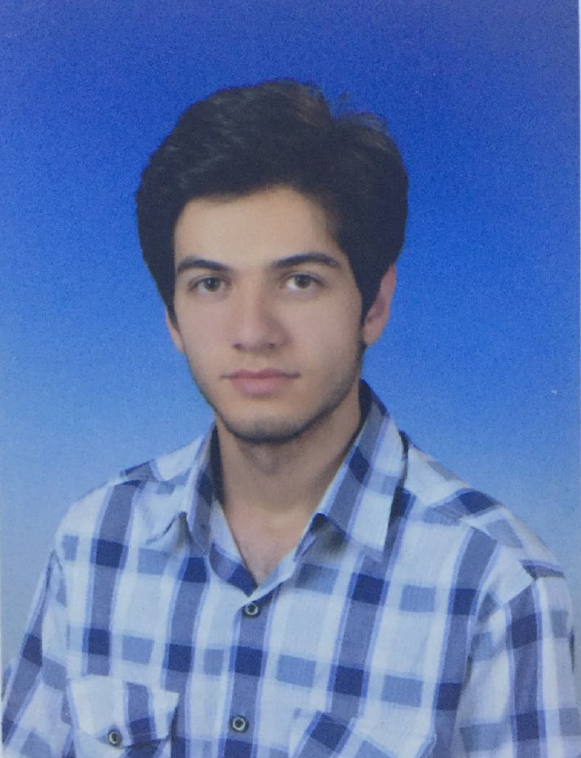
\includegraphics[width=0.8\unitlength]{images/enes_foto}
	\caption{\label{fig:enes_foto} \small Enes Taştan }
\end{figure}

\end{flushright}
\end{minipage}\\[0.4cm]

More information about Enes TAŞTAN can be accessed from his curriculum vitae at APPENDIX.\\[0.4cm]

%--------Erdem---------

\begin{minipage}{0.33\textwidth}
\begin{flushleft} 

\begin{figure}[H]
	\center
	\setlength{\unitlength}{\textwidth} 
	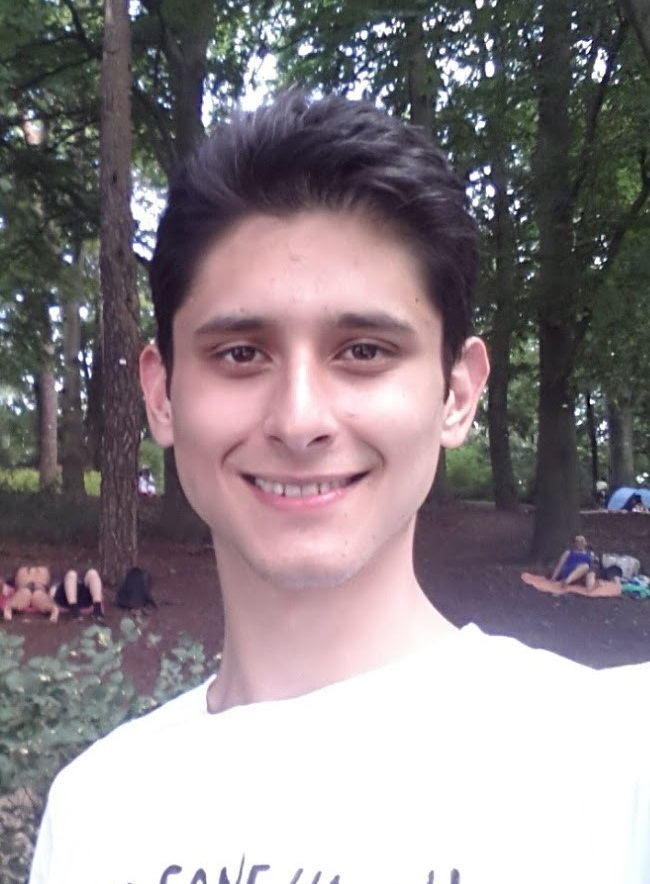
\includegraphics[width=0.8\unitlength]{images/erdem_foto}
	\caption{\label{fig:erdem_foto} \small Erdem TUNA }
\end{figure}

\end{flushleft}
\end{minipage}
\begin{minipage}{0.67\textwidth}
\begin{flushleft} 

	Erdem TUNA can be considered as the name father of the DUAYENLER Ltd. Şti. since He was the one naming their EE302 project group as "Group Duayenler.". Erdem is also long-lasting laboratory and homework partner with Halil since Physics 106 Laboratory. As a graduation student, he chose the \textbf{Computer} option. And as an engineering student, he has specialized in number of topics such as:
	
\begin{itemize}
	\item Static Image Processing (Text Detection etc.)
	\item Programming: Python, C, HTML, CSS 
	\item Interfacing with sensors 
	\item Wireless Communication
\end{itemize}

\end{flushleft}
\end{minipage}\\[0.4cm]

More information about Erdem TUNA can be accessed from his curriculum vitae at APPENDIX.\\[0.4cm]

%---------Halil----------


\begin{minipage}{0.61\textwidth}
\begin{flushleft} 

	Halil TEMURTAŞ, a graduation student, is the fourth co-founder of the DUAYENLER. He is also homework/laboratory partner with Erdem since 2016 and was project partner with Sarper in EE302 project grouyp "Group Duayenler". As a graduation student, he chose the \textbf{Control} option. And as an engineering student, he has specialized in number of topics such as:
	
	
\begin{itemize}
	\item Micro-controllers : Raspberry Pi, Arduino
	\item Device Testing 
	\item Programming Background: Python, C 
	\item System Engineering
\end{itemize}

\end{flushleft}
\end{minipage}
\begin{minipage}{0.38\textwidth}
\begin{flushright}
 
\begin{figure}[H]
	\center
	\setlength{\unitlength}{\textwidth} 
	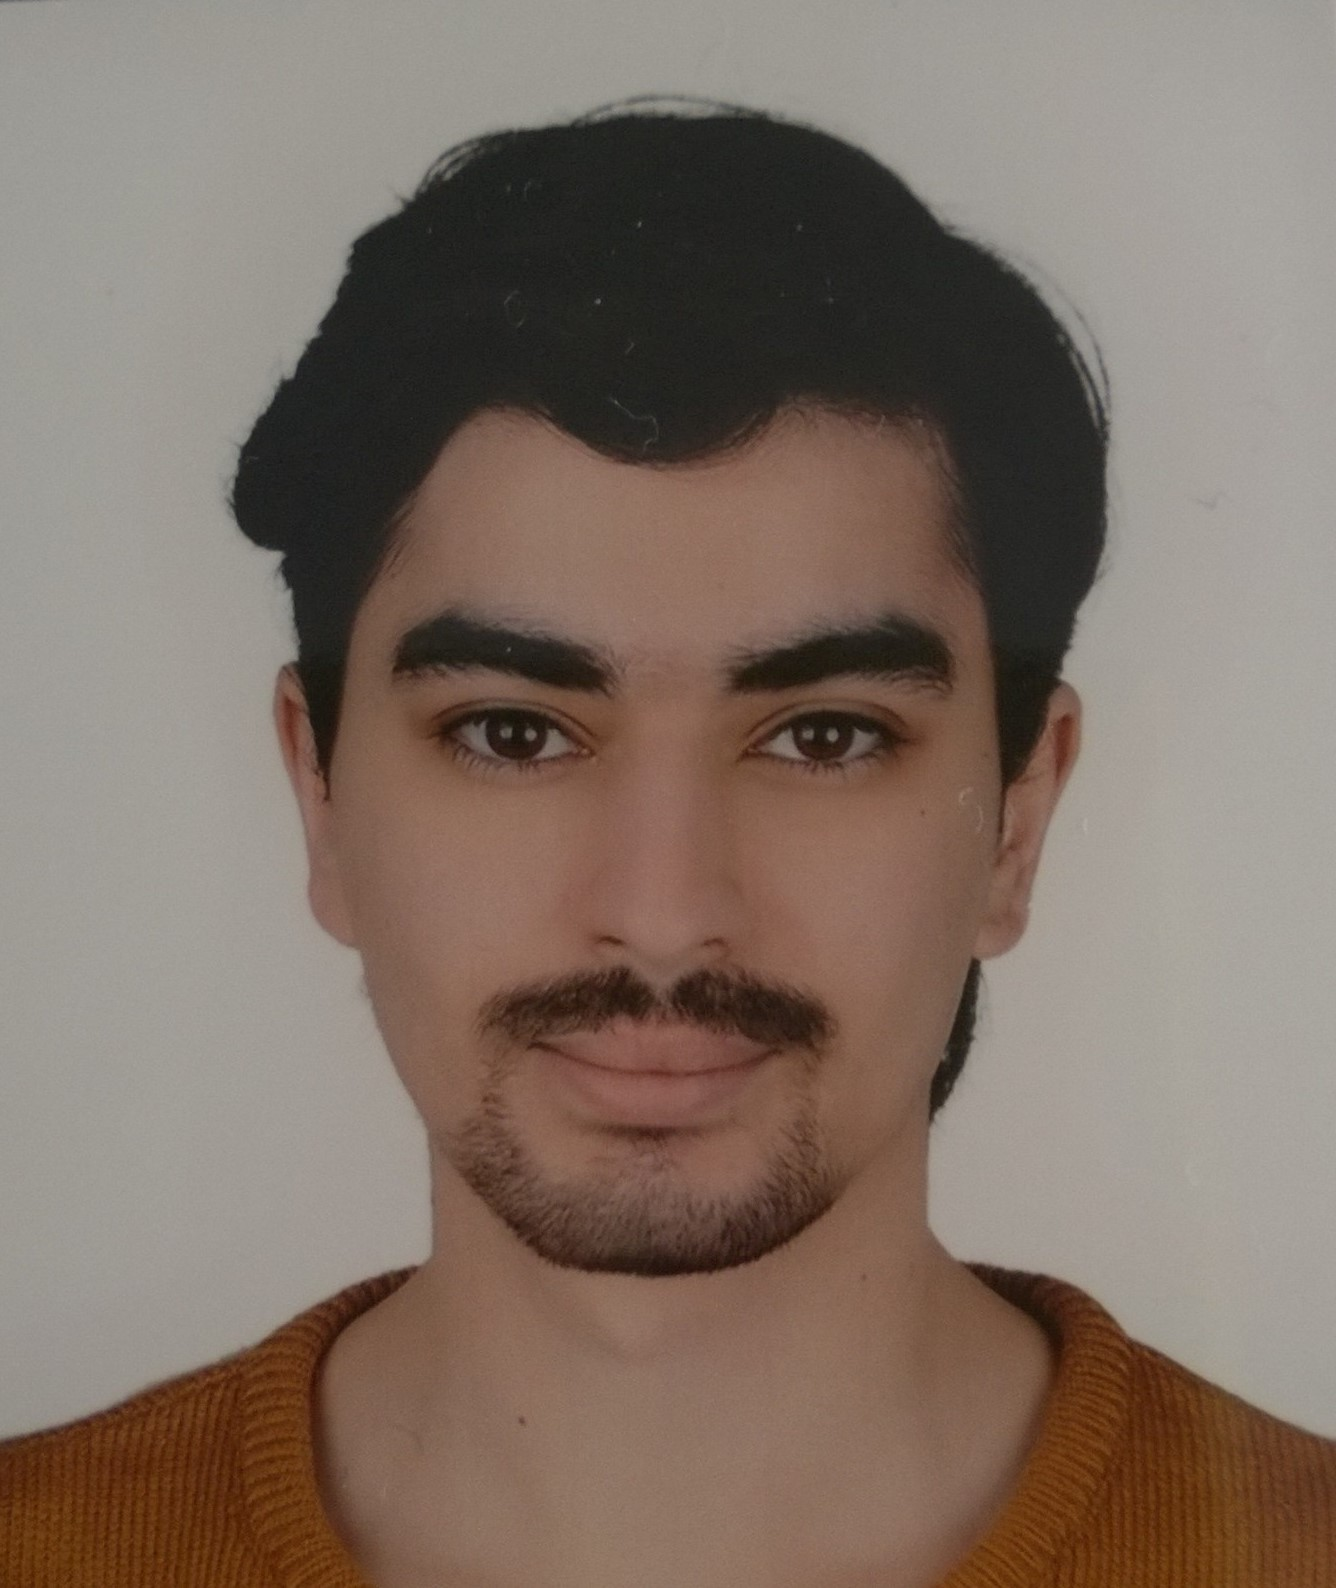
\includegraphics[width=0.7\unitlength]{images/halil_foto}
	\caption{\label{fig:halil_foto} \small Halil TEMURTAŞ }
\end{figure}

\end{flushright}
\end{minipage}\\[0.4cm]

More information about Halil TEMURTAŞ can be accessed from his curriculum vitae at APPENDIX.\\[0.4cm]

%------İlker---------

\begin{minipage}{0.38\textwidth}
\begin{flushleft}

\begin{figure}[H]
	\center
	\setlength{\unitlength}{\textwidth} 
	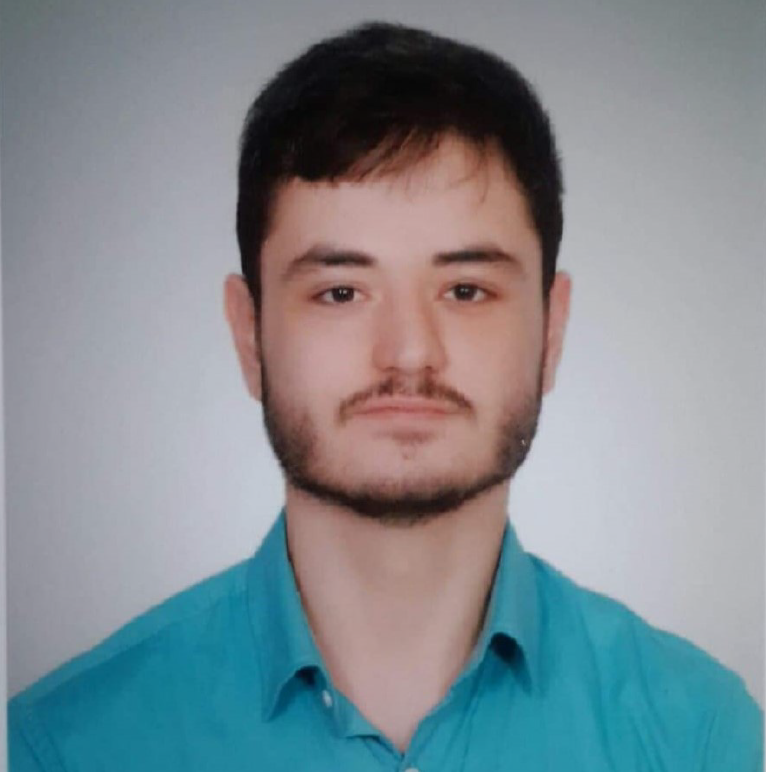
\includegraphics[width=0.7\unitlength]{images/ilker_foto}
	\caption{\label{fig:ilker_foto} \small İlker SAĞLIK }
\end{figure}


\end{flushleft}
\end{minipage}
\begin{minipage}{0.61\textwidth}
\begin{flushleft}

	İlker Sağlık, a graduation student, is the fourth co-founder of the DUAYENLER. He was also a partner with Sarper in one of the third-year laboratory courses. As a graduation student, he chose the \textbf{Computer} option. And as an engineering student, he has specialized in number of topics such as:
		
\begin{itemize}
	\item Plug-in Writer 
	\item Programming Background: Python, C 
	\item Expert LtSpice User
	\item Advance Matlab User
\end{itemize}

\end{flushleft} 
\end{minipage}\\[0.4cm]

More information about İlker SAĞLIK can be accessed from his curriculum vitae at APPENDIX.\\[0.4cm]

%\todo{TODO NOTE}

\section{Description of the Projects}
The analysis of each projects including possible challenges and solutions are given in this section.

\subsection{Devices Competing to Catch Falling Balloons}

In this project, we are supposed to design and construct two robots that try to catch falling balloons before they touch the floor. However, we have some limitations with this design. Firstly, the sizes of the robots must not exceed the upper limit provided us. Secondly, robots are not allowed to touch, push or contact each other. Thirdly, the protection from the interference from robots’ sensors is required.\\

There are two major problems related to this project. First problem is moving the robot to the direction of the balloon. To solve this, a built-in camera on the robots can be utilized. We can take a reference point on the camera, and try to make it aligned with the balloon. However, image processing is highly required. Second problem is the way of catching the balloons. Robot arms or vacuums can be utilized in this step. However, we think the vacuums would be much easier. In overall, image processing and algorithm to make robots tend the direction of balloons avoiding collusion are required.

\subsection{Devices Trying to Score in Each Other’s Goals}
In this project, we need to design a device which can play basically air hokey by remote control (no Wi-Fi) in a hexagonal playground. This project is focusing on RF communication and real-time process. No naked eye and onboard camera requirement video transmission should have no lag and right angle. There are, also, some mechanic problems which are how to respond a ball and how to handle with the stuck ball. Our approach to camera angle is using a servo motor and adding a camera control button to controller, so in every condition of the device, player can observe field properly. For hitting the ball, our consideration has two part using momentum of the ball to respond during the game, so orientation problem can be solved. On the other hand, to solve stuck ball problem and the beginning of the game, we need to push the ball. Therefore, we can add impulsive component to one side. To handle with real-time process, we should have fast algorithm in communication and movement. 

\subsection{Vehicles Chasing Each Other Around a Closed Course with Varying Properties}

In this project, we are required to build a vehicle that can travel around a closed elliptical route as fast as possible. Furthermore, it should stay on the elevated path. At first glance, the main requirement of the vehicle is to have a reliable and quick responsive motion control system. To handle the turns on the path, a differential drive principle can be used as well as direction changing wheels. However, the latter one is hard to build and need to be tested if it is capable of handling the specified path. Another factor that needs to be put attention is the speed of the vehicle. Since it is a race between two vehicles, it is better to come up with the most practical and feasible solutions for the controls system so that the processing load is minimized. After all, the vehicles are required to complete the path in less than 20 seconds.\\

The winner is defined to be the vehicle that can approach to other one from the back less than 5 cm. Therefore, the vehicle should have a function that when the winning event occurs, it can stop the race by so called handshake protocol. The overlooking cameras are not allowed but it is not a feasible way either. It is because processing the image and sending the necessary informations to vehicle so that it performs accurately is too much process and would take longer compared to data coming from sensors onboard. Also, a suspension system might be needed to achieve stability against rough surfaces or disturbances. In addition, there needs to be protection system on the vehicle so that the collision with the other one never occurs.


\subsection{Devices Trying to Extract the Plan of Their Surroundings}
The project requires a mobile vehicle that can travel in a meaningful path such that the device neither crashes any of the obstacles nor the exterior walls but can map the whole playfield accurately. The main limiting factor in the solution is the use of same color for both the obstacles and the exterior wall. This limitation prevents the implementation of a simple color thresholding solution for the object detection with the help of a imaging system such as a camera. A possible way to handle the object detection problem would be to use “shadow games” so that light shades of the color indicate a possible object whereas the dark shades of the color might mean exterior wall. Certainly, mapping the playfield is important as much as object detection. The vehicle should be able to get the distance of it to its environment. \\

The overall solution requires a combination of many steps, mainly, image processing, direction automation with respect to surroundings, an algorithm to create map.


\section{Conclusion}
	In this report, the general information about the DUAYENLER Ltd. Şti. was given and the as co-founders of the company is introduced. Afterwards, four possible Capstone projects were explained from the co-founders perspective in brief details.

Time table for the tasks including the assignment of responsibilities until the submission of the proposal report

%\begin{itemize}
%\item Item
%\item Item
%\end{itemize}

%\begin{figure}[H]
%\center
%\setlength{\unitlength}{\textwidth} 
%
\includegraphics[width=0.7\unitlength]{images/logo1}
%\caption{\label{fig:logo}Logo }
%\end{figure}

%\begin{figure}[H]
%	\setlength{\unitlength}{\textwidth} 
%	\centering
%	\begin{subfigure}{.5\textwidth}
%  		\centering
%  		
\includegraphics[width=0.48\unitlength]{images/logo1}
%  		\caption{\label{fig:logo1}Logo1 }
%	\end{subfigure}%
%	\begin{subfigure}{.5\textwidth}
%  		\centering
%		
\includegraphics[width=0.48\unitlength]{images/logo2}
%  		\caption{\label{fig:logo2}Logo2}
%	\end{subfigure}
%\caption{\label{fig:calisandegree} Small Logos   }
%\end{figure}
	
%\begin{table}[H]
%  \centering
% 
%    \begin{tabular}{c|c|c}
%       $$A$$ & $$B$$ & $$C$$ \\ \hline
%       1 & 2 & 3  \\ \hline
%       2 & 3 & 4  \\ \hline
%       3 & 4 & 5  \\ \hline
%       4 & 5 & 6  
%      
%  \end{tabular}
%  \caption{table}
%  \label{tab:table}
%\end{table}
	
%\begin{table}[H]
%  \centering
% 
%    \begin{tabular}{c|c|c}
%       \backslashbox{$A$}{$a$} & $$\specialcell{ Average deviation \\ after subtracting out the  \\ frequency error }$$ & $$C$$ \\ \hline
%       \multirow{2}{*}{1} & 2 & 3  \\ \cline{2-3}
%        & 3 & 4  \\ \hline
%       3 & \multicolumn{2}{c}{4}  \\ \hline
%       4 & 5 & 6  
%      
%  \end{tabular}
%  \caption{table}
%  \label{tab:table}
%\end{table}

\appendix

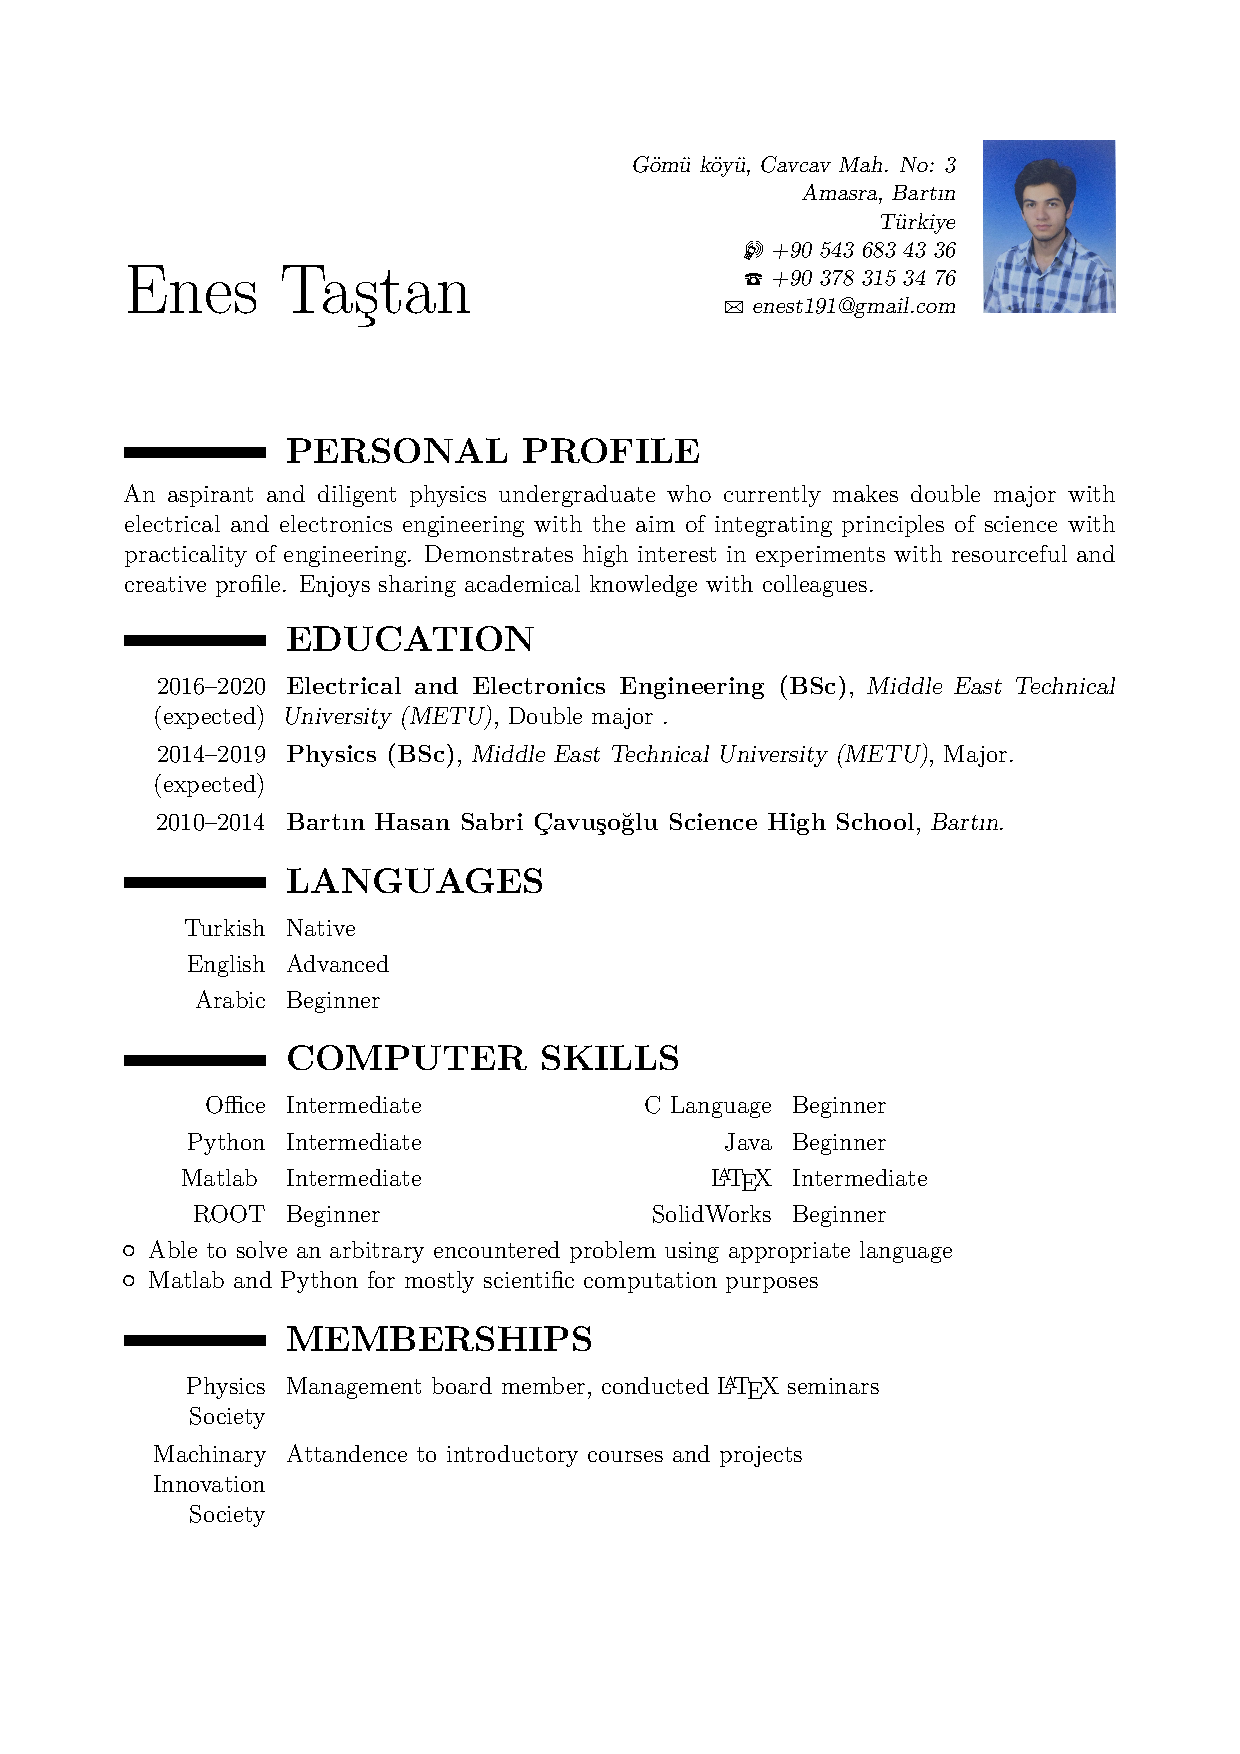
\includepdf[pages=1-2, scale=1.0 ]{CVs/Enes_CV}
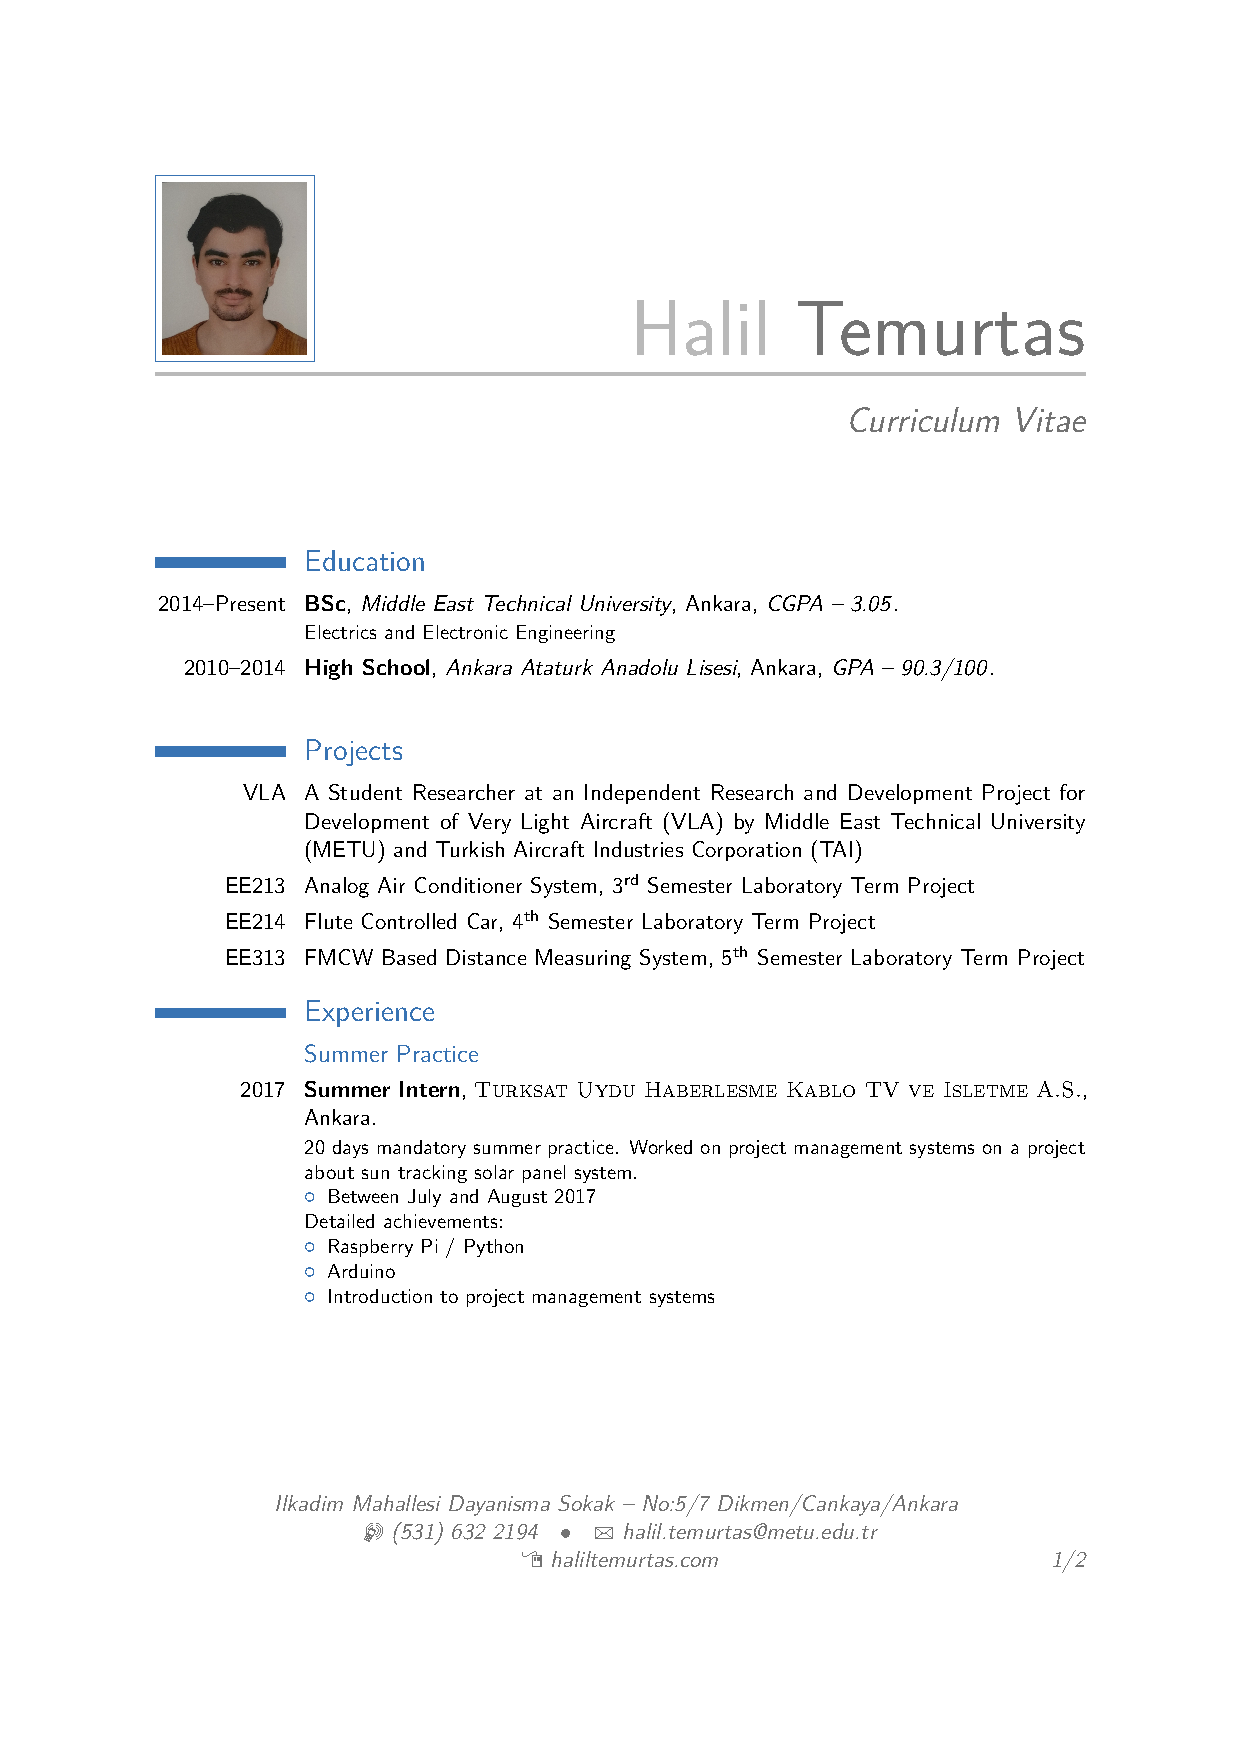
\includepdf[pages=1-2, scale=1.0 ]{CVs/Halil_CV}
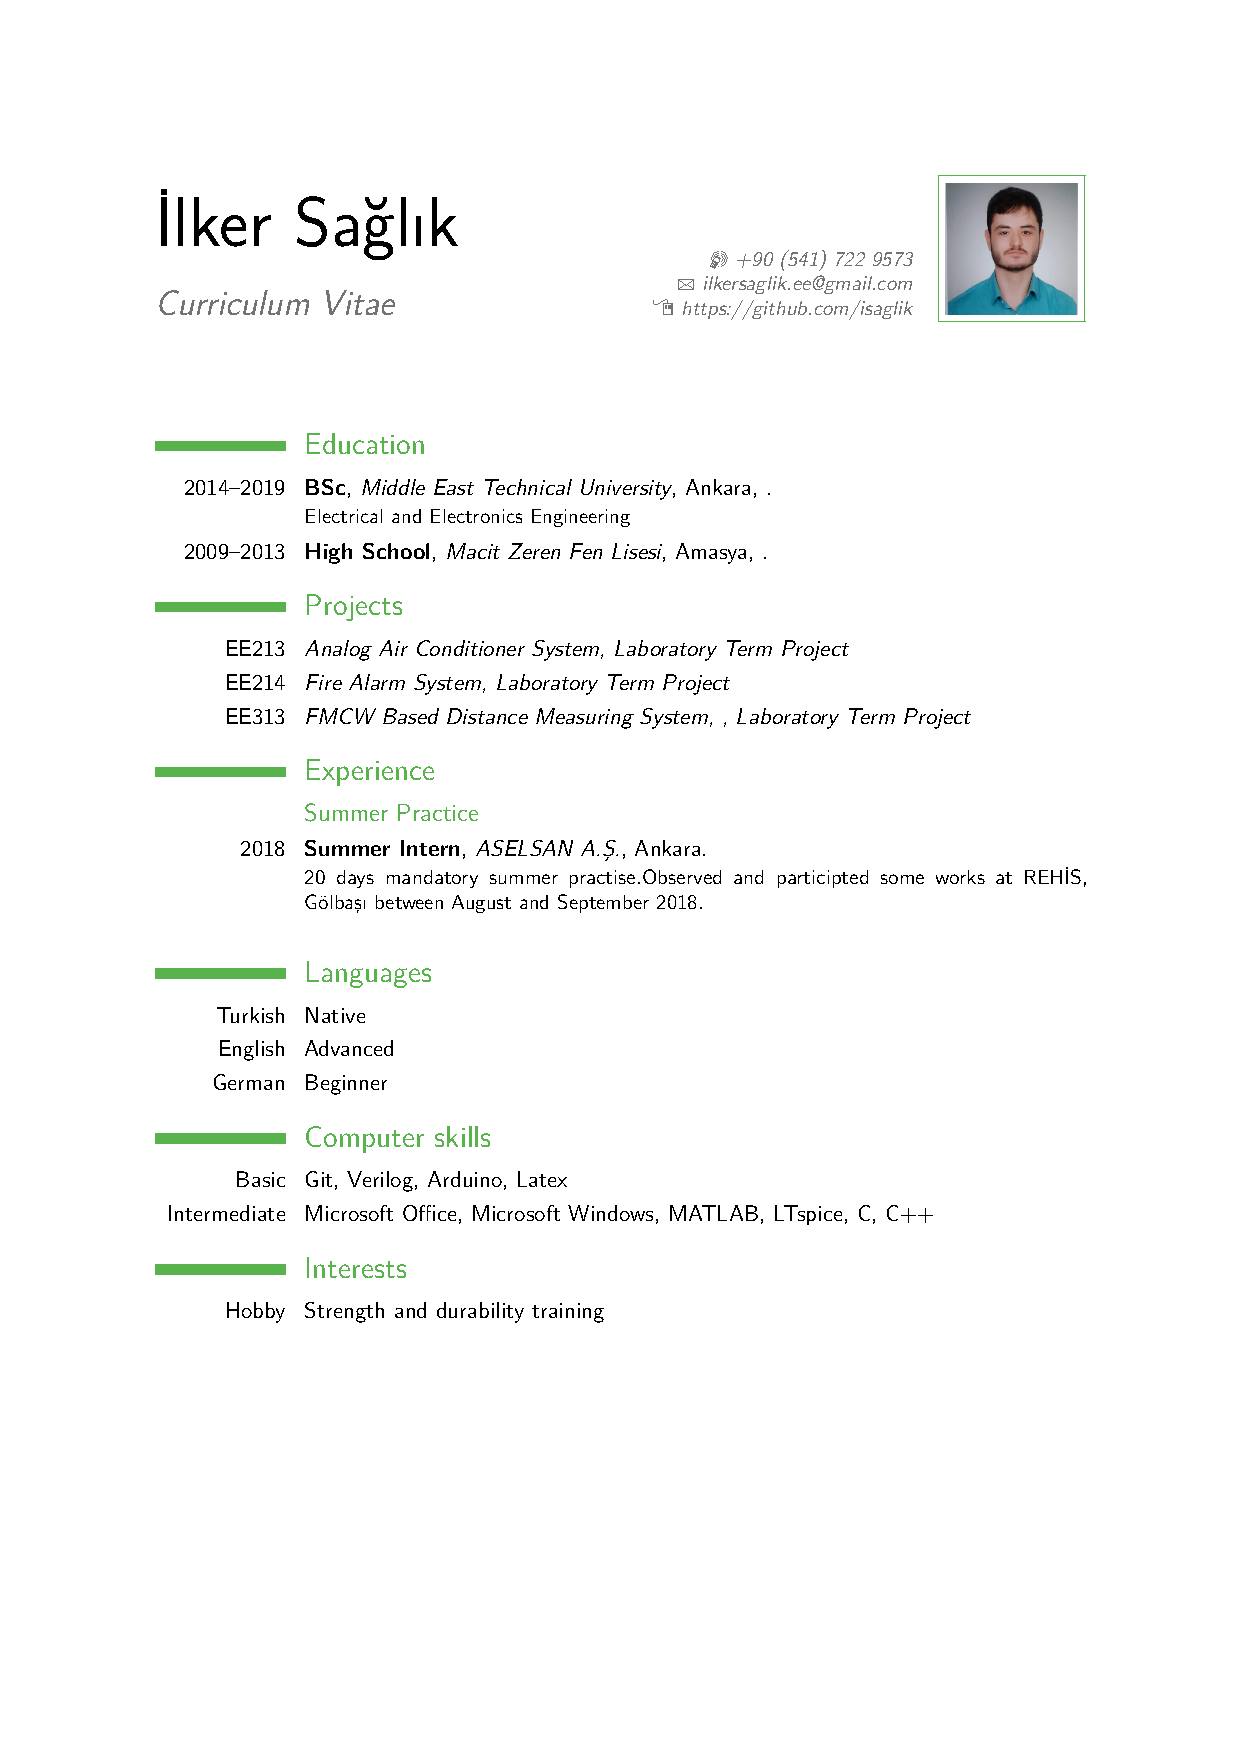
\includepdf[pages=1, scale=1.0 ]{CVs/Ilker_CV}
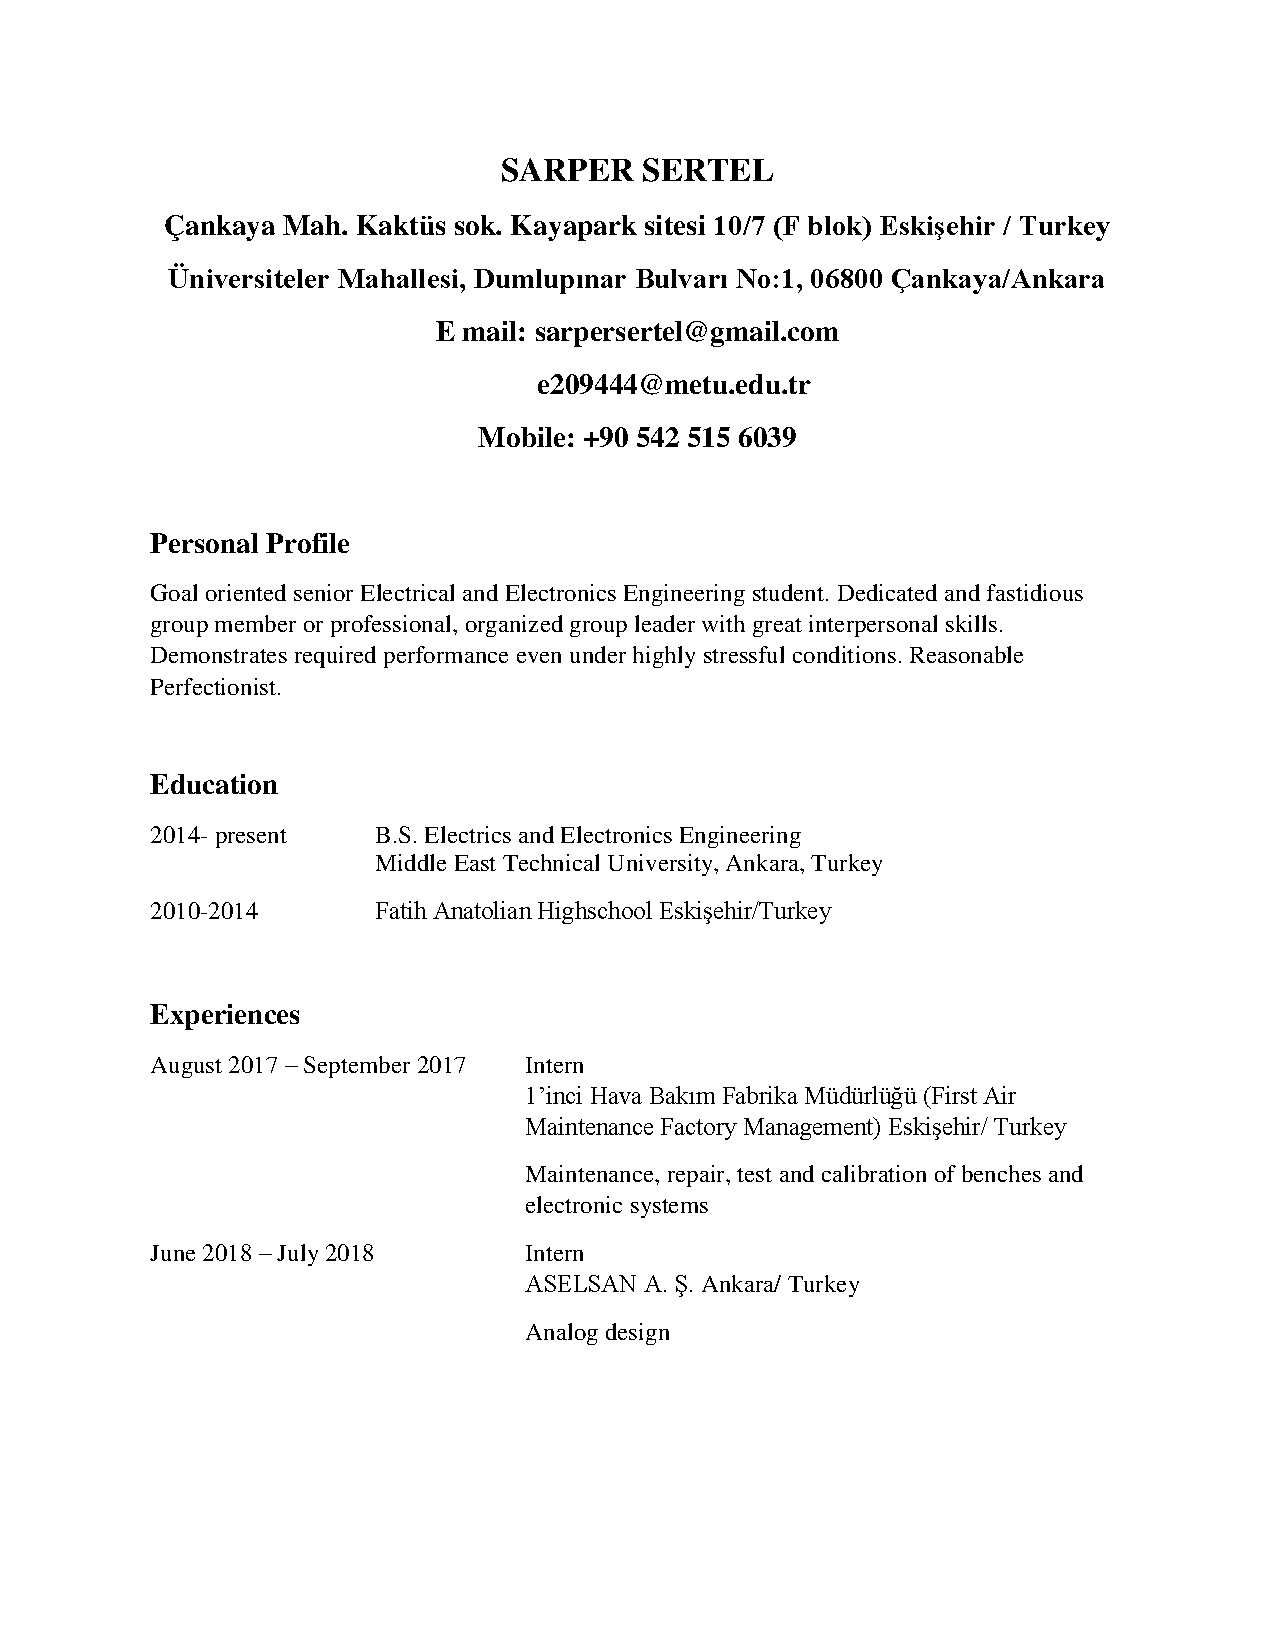
\includepdf[pages=1-2, scale=1.0 ]{CVs/Sarper_CV}




%----samples------
\begin{itemize}
	\item Item
	\item Item
\end{itemize}


\begin{figure}[H]
\centering
\setlength{\unitlength}{\textwidth} 

\includegraphics[width=0.7\unitlength]{images/logo1}
\caption{\label{fig:logo}Logo }
\end{figure}


\begin{figure}[H]
	\setlength{\unitlength}{\textwidth} 
	\centering
	\begin{subfigure}{.5\textwidth}
  		\centering
  		
\includegraphics[width=0.48\unitlength]{images/logo1}
  		\caption{\label{fig:logo1}Logo1 }
	\end{subfigure}%
	\begin{subfigure}{.5\textwidth}
  		\centering
		
\includegraphics[width=0.48\unitlength]{images/logo2}
  		\caption{\label{fig:logo2}Logo2}
	\end{subfigure}
\caption{\label{fig:calisandegree} Small Logos   }
\end{figure}
	
\begin{table}[H]
  \centering
  \caption{table}\label{tab:table1}%table captions must be on top
    \begin{tabular}{c|c|c}
       $$A$$ & $$B$$ & $$C$$ \\ \hline
       1 & 2 & 3  \\ \hline
       2 & 3 & 4  \\ \hline
       3 & 4 & 5  \\ \hline
       4 & 5 & 6     
  \end{tabular}
\end{table}


\begin{table}[H]
  \centering
 
    \begin{tabular}{c|c|c}
       \backslashbox{$A$}{$a$} & $$\specialcell{ Average deviation \\ after subtracting out the  \\ frequency error }$$ & $$C$$ \\ \hline
       \multirow{2}{*}{1} & 2 & 3  \\ \cline{2-3}
        & 3 & 4  \\ \hline
       3 & \multicolumn{2}{c}{4}  \\ \hline
       4 & 5 & 6  
      
  \end{tabular}
  \caption{table}
  \label{tab:table2}
\end{table}
%-----end of samples-----

\end{document}
